\chapter{Visibility and contact representations of planar graphs}

\section{$s-t$ numbering}

\begin{defn}
	An $s - t$ numbering (also called a bipolar orientation) of a graph is an acyclic orientation of its edges which has exactly one source (a vertex with no in-coming arcs) and exactly one sink (a vertex with no out-going arcs).
\end{defn}

\begin{prop}
	Every vertex 2-connected graph has an $s - t$ numbering.
\end{prop}

\begin{proof}
	By induction on adding ears, using the Ear Decomposition Lemma. Given the starting cycle, choose two distinct vertices on it (to be the source and the sink) and orient the cycle as two directed paths from the source to the sink. The loop invariant will be that every vertex lies on a directed path from the source to the sink. When adding an ear, orient it in the direction from the source to the sink if both end-vertices of the ear lie on the same path from the source to the sink. If the end-vertices of the ear lie on different paths from the source to the sink, the ear may be oriented either way (but all of its edges in the same direction).
\end{proof}

\begin{thm}
	Every vertex 2-connected plane graph has an $s - t$ numbering and a noncrossing planar drawing such that
	
	\begin{enumerate}[i)]
		\item every edge is drawn as a $y$-monotone curve (i.e., every horizontal line crosses the drawing of the edge in at most one point), and
		\item the drawing of every edge is oriented upward in the $s - t$ numbering.
	\end{enumerate}
	\label{thm-1}
\end{thm}

This $s - t$ numbering and a corresponding planar drawing can be constructed in polynomial time.

\begin{comm}
	By saying a plane graph it is meant a planar graph with a given noncrossing drawing in the plane, and it is understood that only drawings which are homeomorphic to the given one are considered, including the choice of the outerface.
\end{comm}

\begin{proof}
	By Ear Decomposition Lemma, the given graph $G$ can be constructed from the cycle bounding its outerface by adding ears. Choose two distinct vertices, say $a$ and $b$, on this cycle, place them in the plane so that they have different $y$-coordinates, the coordinate of $a$ being smaller than the coordinate of $b$, orient the two $a - b$ paths forming the cycle from $a$ to $b$ and draw them as $y$-monotone paths from (the drawing of) $a$ to (the drawing of) $b$.
	
	Then continue adding the ears, orienting their edges and adding them to the drawing constructed while keeping the following loop invariant -- the drawing is homeomorphic to the so far constructed part of $G$, it satisfies i) and ii), all vertices have distinct $y$-coordinates, and each face is bounded by two upward oriented paths connecting its vertices with the lowest and the highest $y$-coordinates (we will refer to these paths as the \textit{left} one and the \textit{right} one). Note that i) and ii) together imply that the drawing of any directed path is $y$-monotone.
	
	When an ear is added, it is added inside a face of the so far constructed part of $G$. Direct the edges of the ear in the direction from the vertex with the lower $y$-coordinate to the vertex with the higher one (the end-vertices of the ear belong to the so far constructed part of $G$ and so they have already been drawn). If the end-vertices belong to the same bounding path (the left one or the right one) of the face they should be draw in, draw the ear as a $y$-monotone curve contouring the bounding path. If the end-vertices belong to different bounding paths, draw the ear as a $y$-monotone curve that contours the path which contains the lower endpoint and traverse the face to the other endpoint almost horizontally close to the $y$-coordinate of this other endpoint, in order to avoid crossings with other edges. It is easy to check that the loop invariant of the construction is fulfilled.
\end{proof}

\begin{figure}[!ht]\centering
	\begin{subfigure}{0.45\textwidth}\centering
		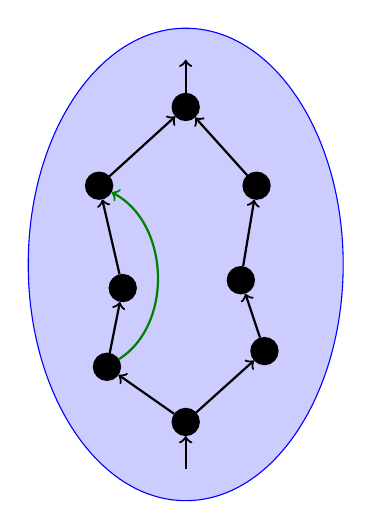
\begin{tikzpicture}[main/.style = {draw, circle, thick, fill}]
			% Draw ellipsoid
			\draw[blue, fill=blue!20] (0,0) ellipse (2 and 3);
			\node[main] (1) at (0,-2) {};
			\node[main] (2) at (-1,-1.3) {};
			\node[main] (3) at (1,-1.1) {};
			\node[main] (4) at (-0.8,-0.3) {};
			\node[main] (5) at (0.7,-0.2) {};
			\node[main] (6) at (-1.1,1) {};
			\node[main] (7) at (0.9,1) {};
			\node[main] (8) at (0,2) {};
			
			\draw[->, thick] (1) edge (2);
			\draw[->, thick] (1) edge (3);
			\draw[->, thick] (2) edge (4);
			\draw[->, thick] (3) edge (5);
			\draw[->, thick] (4) edge (6);
			\draw[->, thick] (5) edge (7);
			\draw[->, thick] (6) edge (8);
			\draw[->, thick] (7) edge (8);
			
			\draw[->, thick] (0, -2.6) -- (1);
			\draw[->, thick] (8) -- (0, 2.6);
			
			\draw[->, thick, color=Green, bend right = 60] (2) edge (6);
		\end{tikzpicture}
	\end{subfigure}
	\begin{subfigure}{0.45\textwidth}\centering
		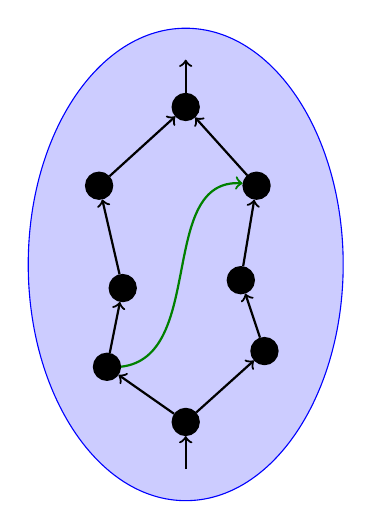
\begin{tikzpicture}[main/.style = {draw, circle, thick, fill}]
			% Draw ellipsoid
			\draw[blue, fill=blue!20] (0,0) ellipse (2 and 3);
			\node[main] (1) at (0,-2) {};
			\node[main] (2) at (-1,-1.3) {};
			\node[main] (3) at (1,-1.1) {};
			\node[main] (4) at (-0.8,-0.3) {};
			\node[main] (5) at (0.7,-0.2) {};
			\node[main] (6) at (-1.1,1) {};
			\node[main] (7) at (0.9,1) {};
			\node[main] (8) at (0,2) {};
			
			\draw[->, thick] (1) edge (2);
			\draw[->, thick] (1) edge (3);
			\draw[->, thick] (2) edge (4);
			\draw[->, thick] (3) edge (5);
			\draw[->, thick] (4) edge (6);
			\draw[->, thick] (5) edge (7);
			\draw[->, thick] (6) edge (8);
			\draw[->, thick] (7) edge (8);
			
			\draw[->, thick] (0, -2.6) -- (1);
			\draw[->, thick] (8) -- (0, 2.6);
			
			\draw[->, thick, color=Green, bend right, out=-50, in=120] (2) edge (7);
		\end{tikzpicture}
	\end{subfigure}
	\caption{An illustration to adding an ear in the construction of an $s-t$ numbering and a corresponding upward drawing.}
\end{figure}

\section{Rectangle visibility representations}

\begin{defn}
	A \textbf{rectangle visibility representation} of a plane graph $G$ is an arrangement of disjoint axes-aligned rectangles in the plane such that the (unions of) horizontal sides of the rectangles correspond to the vertices of $G$, the (unions of) vertical sides to the faces of $G$, and each rectangle corresponds to the edge joining the vertices containing the upper and lower sides of the rectangle, and at the same time to the dual edge joining the faces corresponding to the left and right sides of the rectangle.
\end{defn}

\begin{comm}
	In this section we allow multiple edges without explicitly talking about \\ multigraphs. Moreover, we artificially choose two vertices on the boundary of the outerface and divide the outerface into two faces by "infinite" dummy edges starting in these points.
\end{comm}

\begin{figure}[!ht]\centering
	\begin{subfigure}{0.6\textwidth}\centering
		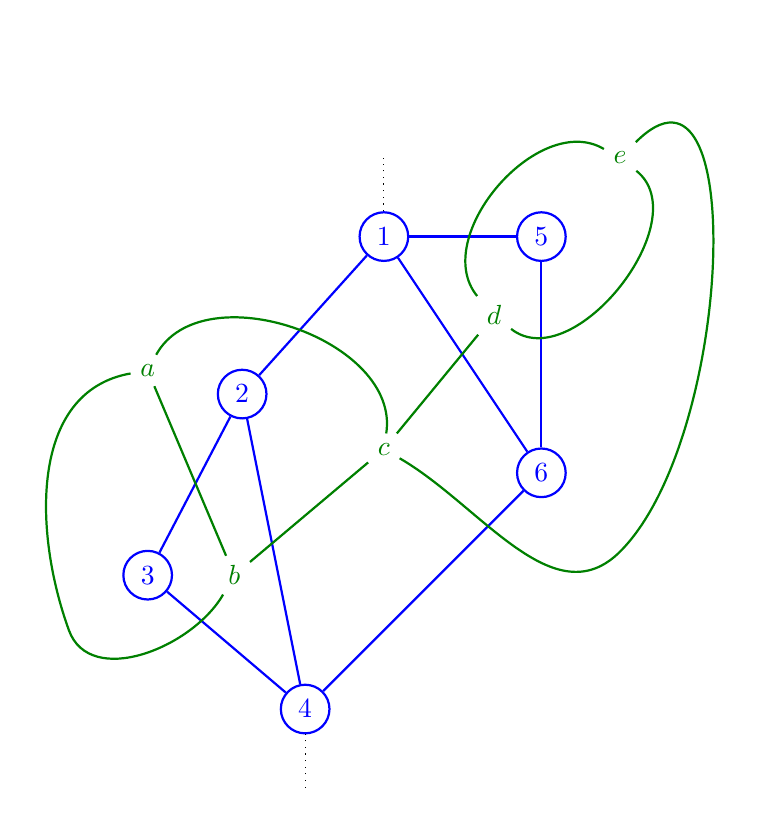
\begin{tikzpicture}[main/.style = {draw, circle, thick, color = Blue}]
			\node[main] (4) at (0,0) {4};
			\node[main] (3) at (-2,1.7) {3};
			\node[main] (6) at (3,3) {6};
			\node[main] (2) at (-0.8,4) {2};
			\node[main] (5) at (3,6) {5};
			\node[main] (1) at (1,6) {1};
			\node[color=Green] (b) at (-0.9, 1.7) {$b$};
			\node[color=Green] (a) at (-2, 4.3) {$a$};
			\node[color=Green] (c) at (1, 3.3) {$c$};
			\node[color=Green] (d) at (2.4, 5) {$d$};
			\node[color=Green] (e) at (4, 7) {$e$};
			\draw[thick, color=Blue] (4) edge (3);
			\draw[thick, color=Blue] (4) edge (2);
			\draw[thick, color=Blue] (4) edge (6);
			\draw[thick, color=Blue] (5) edge (6);
			\draw[thick, color=Blue] (6) edge (1);
			\draw[thick, color=Blue] (2) edge (1);
			\draw[thick, color=Blue] (1) edge (5);
			\draw[thick, color=Blue] (2) edge (3);
			\draw[dotted] (0, -1) -- (4);
			\draw[dotted] (1) -- (1, 7);
			\draw[thick, color=Green] (b) edge (c);
			\draw[thick, color=Green] (d) edge (c);
			\draw[thick, color=Green] (b) edge (a);
			
			\coordinate (6') at (4,2);
			\coordinate (3') at (-3, 1);
			
			\draw[thick, color=Green] (b) to[out = 240, in = -70] (3') to[out = 110, in = 190] (a);
			\draw[thick, color=Green, bend left = 80] (a) edge (c);
			\draw[thick, color=Green] (e) to[out = 45, in = 45] (6') to[out = -135, in = -30] (c);
			\draw[thick, color=Green, bend left = 80] (d) edge (e);
			\draw[thick, color=Green, bend right = 90] (d) edge (e);
		\end{tikzpicture}
	\end{subfigure}
	\begin{subfigure}{0.35\textwidth}\centering
		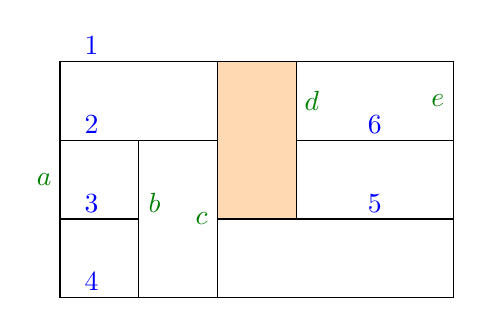
\begin{tikzpicture}
			\draw[black] (0,0) rectangle (1,1);
			\draw[black] (0,1) rectangle (1,2);
			\draw[black] (1,0) rectangle (2,2);
			\draw[black] (2,0) rectangle (5,1);
			\draw[black] (0,2) rectangle (2,3);
			\draw[black, fill=orange!30] (2,1) rectangle (3,3);
			\draw[black] (3,1) rectangle (5,2);
			\draw[black] (3,2) rectangle (5,3);
			\node[Blue] at (0.4, 3.2) {1};
			\node[Blue] at (0.4, 2.2) {2};
			\node[Blue] at (0.4, 1.2) {3};
			\node[Blue] at (0.4, 0.2) {4};
			\node[Green] at (-0.2, 1.5) {$a$};
			\node[Green] at (1.2, 1.2) {$b$};
			\node[Green] at (1.8, 1) {$c$};
			\node[Blue] at (4, 1.2) {5};
			\node[Blue] at (4, 2.2) {6};
			\node[Green] at (3.2, 2.5) {$d$};
			\node[Green] at (4.8, 2.5) {$e$};
		\end{tikzpicture}
	\end{subfigure}
	\caption{An example of a rectangle visibility representation of a planar graph. The highlighted rectangle in the representation corresponds to the primal edge 13 and dual edge $cd$.}
\end{figure}

\begin{thm}
	Every planar vertex 2-connected graph has a rectangle visibility \\ representation.
	\label{thm-2}
\end{thm}

\begin{proof}
	We in fact describe an algorithm how such a representation can be constructed. The bonus is that the construction runs in polynomial time.
\end{proof}

\begin{algorithm}[!ht]
	\caption{RectangleVisibilityRep}
	\begin{algorithmic}[1]
		\Require A planar graph $G$.
		\State Construct an $s - t$ numbering and a corresponding upward planar drawing as in Theorem \ref{thm-1}.
		\State Number the vertices as $1, \dots, n$ according to their $y$-coordinates (1 is the lowest vertex, $n$ is the highest one).
		\State Add a dummy arc from 1 to $n$ drawn to the right of the drawing of $G$, denote by $G'$ the resulting graph.
		\State Construct the dual graph $G^\ast$ to $G'$, and orient its edges so that each edge of $G$ is crossed by its dual edge from left to right, while the added dummy edge is crossed from right to left. Let $n^\ast$ be the number of vertices of $G^\ast$.
		\State Consider a topological sorting of the vertices of $G^\ast$ and name them $A, B, \dots$ according to this sorting.
		\State Take a grid of size $n \times n^\ast$. For a vertex $i$ of $G$, let $\alpha(\beta)$ be the face incident with $i$ with the lowest (highest, respectively) name in the topological sorting of $G^\ast$. Represent $i$ by a horizontal segment on the $i$-th line, starting at the vertical line $\alpha$ and ending on the vertical line $\beta$. For a face $\alpha$ of the drawing of $G'$ (i.e., a vertex of the dual graph $G^\ast$), let $i$ be its lowest vertex and $j$ its highest vertex (with respect to the topological sorting of $G$). Represent $\alpha$ by a segment on the vertical line $\alpha$, starting on the $i$-th horizontal line and ending on the $j$-th one.
		\State \Return this representation.
	\end{algorithmic}
\end{algorithm}

It is, however, necessary to prove that this Algorithm really outputs a rectangle visibility representation of $G$. This is done via a series of claims. The first ones talk about the upward drawing of $G$ constructed in Step 1 and the dual graph $G^\ast$ and its drawing inherited from the drawing of $G$.

\begin{claim}
	Vertex number 1 and vertex number $n$ are both on the boundary of the outerface of $G$ (and also of $G'$). The face that gets the name $A$ is the unbounded face and the face with the highest name, say $Z$, is the other face incident with the dummy edge $1n$.
\end{claim}

\begin{claim}
	The orientation of $G^\ast$ described in Step 4 is acyclic and $A$ is its only source and $Z$ is its only sink. Hence it is indeed an $s - t$ numbering of $G^\ast$. To see this, note first that the edge $AZ$ which crosses the dummy edge $1n$ cannot be involved in any directed cycle, as $A$ is a source and $Z$ is a sink in $G^\ast$. Next observe that a clock-wise oriented cycle in $G^\ast$ would bound a region with at least one vertex of $G$ inside and all edges of $G$ crossing this cycle would be oriented from inside towards the outside of this region, hence, there would necessarily be a source of $G$ in this region, and this would be different from the vertex $1$. Similarly, a counter-clock-wise oriented cycle in $G^\ast$ would bound a region that would contain a sink different from $n$. This would be a contradiction with the assumption that we were working with an $s - t$-numbering of $G$. Finally, a source different from $A$ (a sink different from $Z$) in $G^\ast$ would yield a directed cycle on the boundary of this face of $G$. A contradiction again.
\end{claim}

\begin{claim}
	The boundary of every face $\alpha$ of $G$ consists of two directed paths, the left one and the right one, both connecting the vertex of the lowest number to the vertex of the highest number among the vertices of this face. We have seen this in the proof of Theorem \ref{thm-1}.
\end{claim}

\begin{claim}
	For every vertex $i$ of $G, i \neq 1, n$, the faces incident with $i$ induce two directed paths in $G^\ast$,
	both connecting the face to the left of $i$ to the face lying to the right of $i$, one of the paths passing
	through the faces for which $i$ is their topmost vertex, the other one passing through the faces for which
	$i$ is their lowest vertex. See Fig. \ref{fig-3} right.
	\label{claim-4}
\end{claim}

\begin{figure}[!ht]
	\begin{subfigure}{0.45\textwidth}\centering
		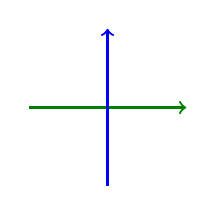
\begin{tikzpicture}
			\draw[->, color=Green, thick] (0,0) -- (2,0);
			\draw[->, color=Blue, thick] (1, -1) -- (1, 1);
		\end{tikzpicture}
		\caption{Orientation of the dual edges.}
	\end{subfigure}
	\begin{subfigure}{0.45\textwidth}\centering
		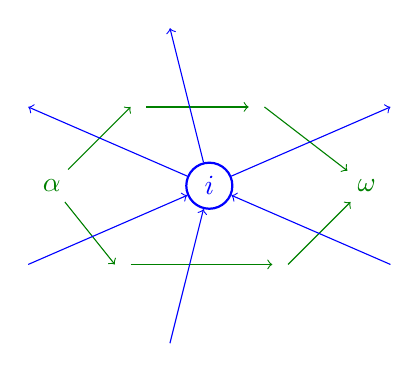
\begin{tikzpicture}
			\node[draw, circle, Blue, thick] (i) at (0,0) {$i$};
			\node[Green, thick] (a) at (-2, 0) {$\alpha$};
			\node[Green, thick] (w) at (2,0) {$\omega$};
			\draw[->, Green] (a) -- (-1, 1);
			\draw[->, Green] (-0.8,1) -- (0.5, 1);
			\draw[->, Green] (0.7, 1) -- (w);
			\draw[->, Green] (a) -- (-1.2, -1);
			\draw[->, Green] (-1, -1) -- (0.8, -1);
			\draw[->, Green] (1, -1) -- (w);
			\draw[->, Blue] (i) -- (-0.5, 2);
			\draw[->, Blue] (-0.5, -2) -- (i);
			\draw[->, Blue] (i) -- (-2.3, 1);
			\draw[->, Blue] (-2.3, -1) -- (i);
			\draw[->, Blue] (i) -- (2.3, 1);
			\draw[->, Blue] (2.3, -1) -- (i);
		\end{tikzpicture}
		\caption{An example to the statement of Claim \ref{claim-4}.}
	\end{subfigure}
	\caption{Examples for claims.}
	\label{fig-3}
\end{figure}

In the next claims we prove that the collection of segments constructed in Step 6 defines a rectangle visibility representation of $G$.

\begin{claim}
	Let $i$ be a vertex of $G, i \neq 1, n$. Let $\alpha$ and $\omega$ be the faces to the left and to the right of $i$, respectively. Then the (horizontal) segment $i$ touches the vertical segment for $\alpha$ from the right, it touches the vertical segment for $\beta$ from the left, it is touched by the segments representing the faces lying on the upper path from $\alpha$ to $\beta$ in $G^\ast$ from above, and it is touched by the faces lying on the lower path from $\alpha$ to $\beta$ in $G^\ast$ from below. The segment representing vertex $1$ spans the whole range from $A$ to $Z$ and is only touched by vertical segments from above, while the segment representing $n$ is only touched by vertical segments from below, and also spans the whole range from $A$ to $Z$.
	\label{claim-5}
\end{claim}

\begin{claim}
	Let $\alpha$ be an inner face of $G$, i.e., a face not incident with the dummy edge $1n$. The vertical segment representing $\alpha$ touches the horizontal segment representing its lowest vertex from above, it touches the segment representing its topmost vertex from below, it is touched by the segments representing the vertices on the left boundary path of $\alpha$ from the left and it is touched by the segments representing the vertices on the right boundary path of $\alpha$ from the right. The segment representing $A$ is touched only from right, while the segment representing $Z$ is touched only from left, always by the appropriate horizontal segments.
	\label{claim-6}
\end{claim}

\begin{figure}[!ht]
	\begin{subfigure}{.25\textwidth}\centering
		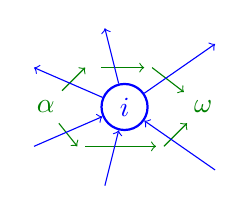
\begin{tikzpicture}
			\node[draw, circle, Blue, thick] (i) at (0,0) {$i$};
			\node[Green, thick] (a) at (-1, 0) {$\alpha$};
			\node[Green, thick] (w) at (1,0) {$\omega$};
			\draw[->, Green] (a) -- (-0.5, 0.5);
			\draw[->, Green] (-0.3,0.5) -- (0.25, 0.5);
			\draw[->, Green] (0.35, .5) -- (w);
			\draw[->, Green] (a) -- (-.6, -.5);
			\draw[->, Green] (-.5, -.5) -- (0.4, -.5);
			\draw[->, Green] (.5, -.5) -- (w);
			\draw[->, Blue] (i) -- (-0.25, 1);
			\draw[->, Blue] (-0.25, -1) -- (i);
			\draw[->, Blue] (i) -- (-1.15, .5);
			\draw[->, Blue] (-1.15, -.5) -- (i);
			\draw[->, Blue] (i) -- (1.15, .8);
			\draw[->, Blue] (1.15, -.8) -- (i);
		\end{tikzpicture}
	\end{subfigure}
	\begin{subfigure}{.2\textwidth}\centering
		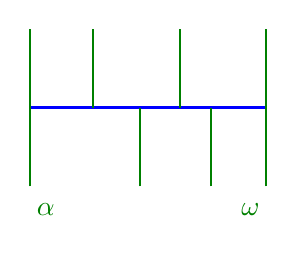
\begin{tikzpicture}
			\draw[thick, Blue] (0,0) -- (3,0);
			\draw[thick, Green] (0,-1) -- (0,1);
			\draw[thick, Green] (3,-1) -- (3,1);
			\draw[thick, Green] (.8,0) -- (.8,1);
			\draw[thick, Green] (1.9,0) -- (1.9,1);
			\draw[thick, Green] (1.4,-1) -- (1.4,0);
			\draw[thick, Green] (2.3,-1) -- (2.3,0);
			\node[Green] at (.2, -1.3) {$\alpha$};
			\node[Green] at (2.8, -1.3) {$\omega$};
		\end{tikzpicture}
	\end{subfigure}
	\begin{subfigure}{.25\textwidth}\centering
		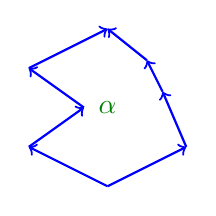
\begin{tikzpicture}
			\draw[->, thick, Blue] (0,0) -- (-1, .5);
			\draw[->, thick, Blue] (-1, .5) -- (-.3, 1);
			\draw[->, thick, Blue] (-.3, 1) -- (-1, 1.5);
			\draw[->, thick, Blue] (-1, 1.5) -- (0, 2);
			\draw[->, thick, Blue] (0,0) -- (1, .5);
			\draw[->, thick, Blue] (1, .5) -- (.7, 1.2);
			\draw[->, thick, Blue] (.7, 1.2) -- (.5, 1.6);
			\draw[->, thick, Blue] (.5, 1.6) -- (0,2);
			\node[Green, thick] at (0,1) {$\alpha$};
		\end{tikzpicture}
	\end{subfigure}
	\begin{subfigure}{.2\textwidth}\centering
		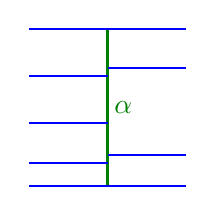
\begin{tikzpicture}
			\draw[Green, thick] (0,0) -- (0,2);
			\draw[Blue, thick] (-1,0) -- (1,0);
			\draw[Blue, thick] (-1,2) -- (1,2);
			\draw[Blue, thick] (-1,.3) -- (0,.3);
			\draw[Blue, thick] (-1,.8) -- (0,.8);
			\draw[Blue, thick] (-1,1.4) -- (0,1.4);
			\draw[Blue, thick] (0,.4) -- (1,.4);
			\draw[Blue, thick] (0,1.5) -- (1,1.5);
			\node[Green, thick] at (0.2, 1) {$\alpha$};
		\end{tikzpicture}
	\end{subfigure}
	\caption{Illustration to Claims \ref{claim-5} and \ref{claim-6}.}
\end{figure}

\begin{claim}
	For every edge $ij$ of $G$, let $\alpha\beta$ be its dual edge. Then the segments representing $i, j, \alpha$ and $\beta$ bound a rectangle in the representation.
	\label{claim-7}
\end{claim}

\begin{claim}
	No two segments constructed in Step 6 cross each other. For suppose segment $j$ crosses segment $\alpha$. By the way the segments are constructed, this means that there exist vertices $i, k, i < j < k$, and $\beta, \gamma, \beta < \alpha < \gamma$, such that $i$ is the lowest and $k$ the topmost vertex of face $\alpha$ and $\beta$ is the left and $\gamma$ the right face incident with $j$. Consider the upward drawing of $G$ and the horizontal stripe of vertices with their $y$-coordinates between $i$ and $k$. The face $\alpha$ spans this stripe from its bottom to its top lines, and thus it lies either to the left or to the right of vertex $i$. Suppose it is to the left. The horizontal ray starting in vertex $i$ and pointing to the left passes first through the face $\beta$ and then crosses several faces until it finally crosses $\alpha$. Since all edges of $G$ it crosses on this way are directed upward, these faces form a path directed from $\alpha$ to $\beta$ in $G^\ast$, which means that $\alpha < \beta$ in the topological sorting of $G^\ast$. Which is a contradiction.
	\label{claim-8}
\end{claim}

\begin{figure}
	\begin{subfigure}{.45\textwidth}\centering
		\begin{tikzpicture}
			\draw[thick, Green] (0,0) -- (0,3);
			\draw[thick, Blue] (-1.5,1.5) -- (1.5, 1.5);
			\draw[dotted] (-1.5, -.2) -- (-1.5, 3.2);
			\draw[dotted] (1.5, -.2) -- (1.5, 3.2);
			\draw[dotted] (-1.7, 0) -- (1.7, 0);
			\draw[dotted] (-1.7, 3) -- (1.7, 3);
			
			\node[Green] at (.3, .2) {$\alpha$};
			\node[Blue] at (1.2, 1.8) {$j$};
			\node[Blue] at (1.9, 0) {$i$};
			\node[Blue] at (1.9, 3) {$k$};
			\node[Green] at (-1.2, -.3) {$\beta$};
			\node[Green] at (1.2, -.3) {$\gamma$};
		\end{tikzpicture}
	\end{subfigure}
	\begin{subfigure}{.45\textwidth}\centering
		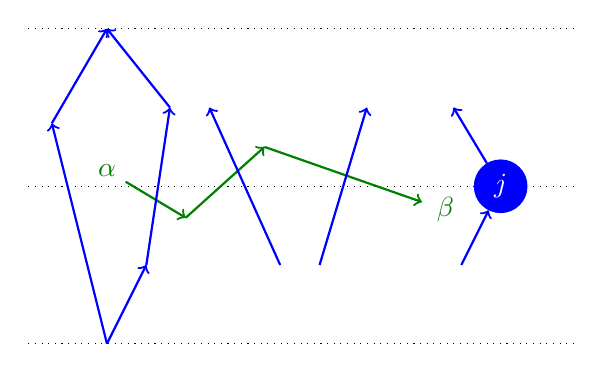
\begin{tikzpicture}
			\draw[dotted] (0,0) -- (7,0);
			\draw[dotted] (0,2) -- (7,2);
			\draw[dotted] (0,-2) -- (7,-2);
			\node[Green] (a) at (1, 0.2) {$\alpha$};
			\draw[->, thick, Green] (a) -- (2, -.4);
			\draw[->, thick, Green] (2, -.4) -- (3, .5);
			\draw[->, thick, Green] (3, .5) -- (5, -.2);
			\node[Green] (b) at (5.3, -.3) {$\beta$};
			\node[draw, circle, Blue, fill] (j) at (6, 0) {\textcolor{white}{$j$}};
			\draw[->, Blue, thick] (5.5, -1) -- (j);
			\draw[->, Blue, thick] (j) -- (5.4, 1);
			\draw[->, thick, Blue] (3.7, -1) -- (4.3,1);
			\draw[->, thick, Blue] (3.2, -1) -- (2.3,1);
			\draw[->, thick, Blue] (1.5, -1) -- (1.8,1);
			\draw[->, thick, Blue] (1,-2) -- (1.5, -1);
			\draw[->, thick, Blue] (1.8, 1) -- (1,2);
			\draw[->, thick, Blue] (1,-2) -- (.3, .8);
			\draw[->, thick, Blue] (.3, .8) -- (1,2);
		\end{tikzpicture}
	\end{subfigure}
	\caption{An illustration to Claim \ref{claim-8}.}
\end{figure}

\begin{claim}
	The rectangles from Claim \ref{claim-7} are disjoint and fill in the base rectangle formed by segments $A, Z, 1, n$. This now follows from the previous claims. And this means that we have indeed constructed a rectangle visibility representation of $G$.
\end{claim}

\begin{figure}[!ht]
	\begin{subfigure}{0.53\textwidth}\centering
		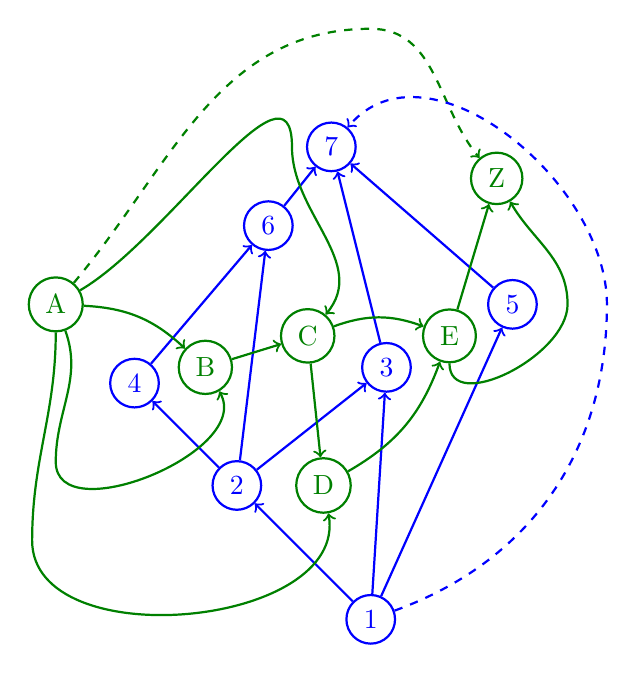
\begin{tikzpicture}[be/.style = {thick, Blue, ->}, ge/.style = {thick, Green, ->},
			bn/.style = {Blue, thick, circle, draw}, gn/.style = {Green, thick, circle, draw}]
			\node[bn] (1) at (0,0) {1};
			\node[bn] (2) at (-1.7, 1.7) {2};
			\node[bn] (3) at (.2, 3.2) {3};
			\node[bn] (4) at (-3, 3) {4};
			\node[bn] (5) at (1.8, 4) {5};
			\node[bn] (6) at (-1.3, 5) {6};
			\node[bn] (7) at (-.5, 6) {7};
			\node[gn] (A) at (-4, 4) {A};
			\node[gn] (B) at (-2.1, 3.2) {B};
			\node[gn] (C) at (-.8, 3.6) {C};
			\node[gn] (D) at (-.6, 1.7) {D};
			\node[gn] (E) at (1, 3.6) {E};
			\node[gn] (Z) at (1.6, 5.6) {Z};
			\draw[be] (1) -- (2);
			\draw[be] (1) -- (3);
			\draw[be] (1) -- (5);
			\draw[be] (2) -- (4);
			\draw[be] (2) -- (6);
			\draw[be] (2) -- (3);
			\draw[be] (5) -- (7);
			\draw[be] (3) -- (7);
			\draw[be] (6) -- (7);
			\draw[be] (4) -- (6);
			\draw[ge, bend left = 20] (A) edge (B);
			\draw[ge] (B) -- (C);
			\draw[ge] (C) -- (D);
			\draw[ge] (E) -- (Z);
			\draw[ge, bend right = 20] (D) edge (E);
			\draw[ge, bend left = 20] (C) edge (E);
			\draw[ge] (A) to[out=290, in=90] (-4, 2) to[out=270, in=300] (B);
			\draw[ge] (A) to[out=270, in=90] (-4.3, 1) to[out=270, in=280] (D);
			\draw[ge] (A) to[out=30, in=90] (-1, 6) to[out=270, in=50] (C);
			\draw[ge] (E) to[out=270, in=270] (2.5, 4) to[out=90, in=300] (Z);
			\draw[ge, dashed] (A) to[out=50, in=180] (0, 7.5) to[out=0, in=130] (Z);
			\draw[be, dashed] (1) to[out=20, in=270] (3, 4) to[out=90, in=50] (7);
		\end{tikzpicture}
	\end{subfigure}
	\begin{subfigure}{0.45\textwidth}\centering
		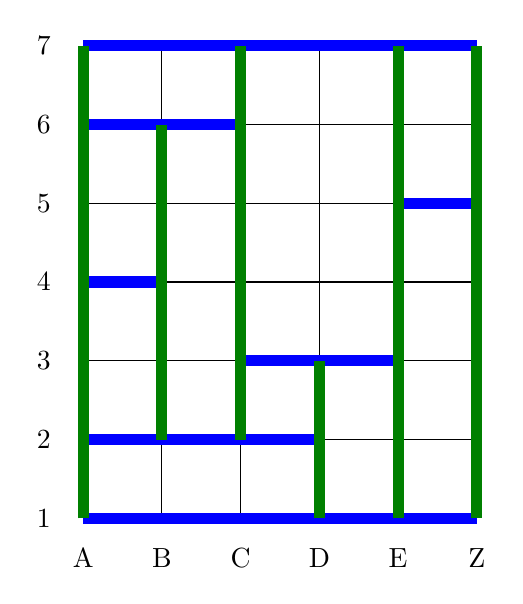
\begin{tikzpicture}[b/.style = {line width = 4, Blue}, g/.style = {line width = 4, Green}]
			\draw (1,1) -- (1,7);
			\draw (2,1) -- (2,7);
			\draw (3,1) -- (3,7);
			\draw (4,1) -- (4,7);
			\draw (5,1) -- (5,7);
			\draw (6,1) -- (6,7);
			\draw (1,1) -- (6,1);
			\draw (1,2) -- (6,2);
			\draw (1,3) -- (6,3);
			\draw (1,4) -- (6,4);
			\draw (1,5) -- (6,5);
			\draw (1,6) -- (6,6);
			\draw (1,7) -- (6,7);
			\draw[b] (1,1) -- (6,1);
			\draw[b] (1,2) -- (4,2);
			\draw[b] (3,3) -- (5,3);
			\draw[b] (1,4) -- (2,4);
			\draw[b] (5,5) -- (6,5);
			\draw[b] (1,6) -- (3,6);
			\draw[b] (1,7) -- (6,7);
			\draw[g] (1,1) -- (1,7);
			\draw[g] (2,2) -- (2,6);
			\draw[g] (3,2) -- (3,7);
			\draw[g] (4,1) -- (4,3);
			\draw[g] (5,1) -- (5,7);
			\draw[g] (6,1) -- (6,7);
			\node at (.5, 1) {1};
			\node at (.5, 2) {2};
			\node at (.5, 3) {3};
			\node at (.5, 4) {4};
			\node at (.5, 5) {5};
			\node at (.5, 6) {6};
			\node at (.5, 7) {7};
			\node at (1,.5) {A};
			\node at (2,.5) {B};
			\node at (3,.5) {C};
			\node at (4,.5) {D};
			\node at (5,.5) {E};
			\node at (6,.5) {Z};
		\end{tikzpicture}
	\end{subfigure}
	\caption{An overview of the construction by Algorithm RectangleVisibilityRep.}
\end{figure}

\section{Grid Contact graphs}

\begin{defn}
	A graph is a \textbf{Grid Intersection graph} if it has an intersection \\ representation by vertical and horizontal segments in which no two segments of the same direction share a point (in other words, all vertical, as well as all horizontal, segments are pairwise disjoint). A graph is a \textbf{Grid Contact} graph if it has a Grid Intersection representation in which no two segments cross, i.e., any two non-disjoint segments only touch each other.
\end{defn}

\begin{prop}
	Every grid intersection graph is bipartite. Moreover, every grid contact graph is planar.
\end{prop}

\begin{proof}
	The first claim is a simple observation. For the second claim, note that grid contact graphs form a subclass of triangle-free contact graphs of arc-connected regions in the plane. All such graphs are planar, since a non-crossing drawing can be constructed from a contact representation by selecting a point inside each region to represent its vertex, and connecting it to the contact points with the adjacent regions by curves inside the region.
\end{proof}

\begin{thm}
	Every planar bipartite graph is a grid contact graph.
	\label{thm-3}
\end{thm}

\begin{proof}
	Given a planar bipartite graph $G = (A \cup B, E)$, consider a non-crossing drawing and extend it to a non-crossing drawing of a supergraph $G' = (A' \cup B' , E')$ such that
	
	\begin{itemize}
		\item $G$ is an induced subgraph of $G'$,
		\item every face of the drawing of $G'$ is bounded by a cycle of length 4 (i.e., $G'$ is a so called quadrangulation),
		\item every vertex of $G'$ has degree greater than $2$, and
		\item no vertex of $B$ is on the boundary of the outerface of $G'$. 
	\end{itemize}
	
	Then construct the graph $\bar{G} = (A', \bar{E})$ by putting $\bar{E}$ the diagonals of the faces of $G'$ connecting their $A'$-vertices. It can be easily seen that $G$ is vertex 2-connected and that the faces of $\bar{G}$ are in 1-1 correspondence with the vertices of $B'$. Thus the segments of a rectangle visibility representation of $\bar{G}$ constructed as in the proof of Theorem \ref{thm-2} form a grid contact representation of $G'$ . Note the technical detail that the vertex (of $B'$) that corresponds to the outerface of $\bar{G}$ is represented by two vertical segments, not one. But this vertex does not belong to $B$, and so the segments corresponding to the vertices of $G$ form a grid contact representation of $G$.
\end{proof}

\begin{figure}[!ht]
	\begin{subfigure}{0.45\textwidth}\centering
		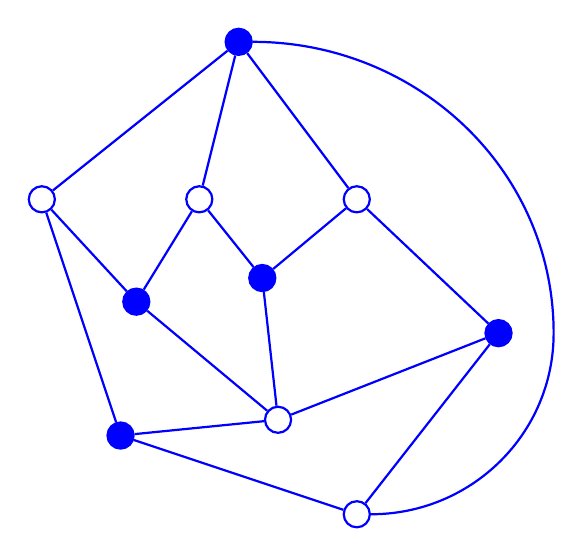
\begin{tikzpicture}[main/.style = {draw, circle, thick, Blue},
			edge/.style = {thick, Blue},
			fil/.style = {thick, fill, draw, circle, Blue}]
			\node[main] (1) at (0,0) {};
			\node[fil] (2) at (1.8, 2.3) {};
			\node[fil] (3) at (-3, 1) {};
			\node[main] (4) at (-1, 1.2) {};
			\node[fil] (5) at (-1.2, 3) {};
			\node[fil] (6) at (-2.8, 2.7) {};
			\node[main] (7) at (-4, 4) {};
			\node[main] (8) at (-2, 4) {};
			\node[main] (9) at (0, 4) {};
			\node[fil] (10) at (-1.5, 6) {};
			\draw[edge] (1) -- (2);
			\draw[edge] (1) -- (3);
			\draw[edge] (3) -- (4);
			\draw[edge] (2) -- (4);
			\draw[edge] (4) -- (5);
			\draw[edge] (4) -- (6);
			\draw[edge] (2) -- (9);
			\draw[edge] (9) -- (10);
			\draw[edge] (8) -- (10);
			\draw[edge] (7) -- (10);
			\draw[edge] (3) -- (7);
			\draw[edge] (6) -- (7);
			\draw[edge] (5) -- (8);
			\draw[edge] (6) -- (8);
			\draw[edge] (5) -- (9);
			\draw[edge] (1) to[out=0, in=270] (2.5, 2.3) to[out=90, in=0] (10);
		\end{tikzpicture}
		\caption{The graph $G'$.}
	\end{subfigure}
	\begin{subfigure}{0.53\textwidth}\centering
		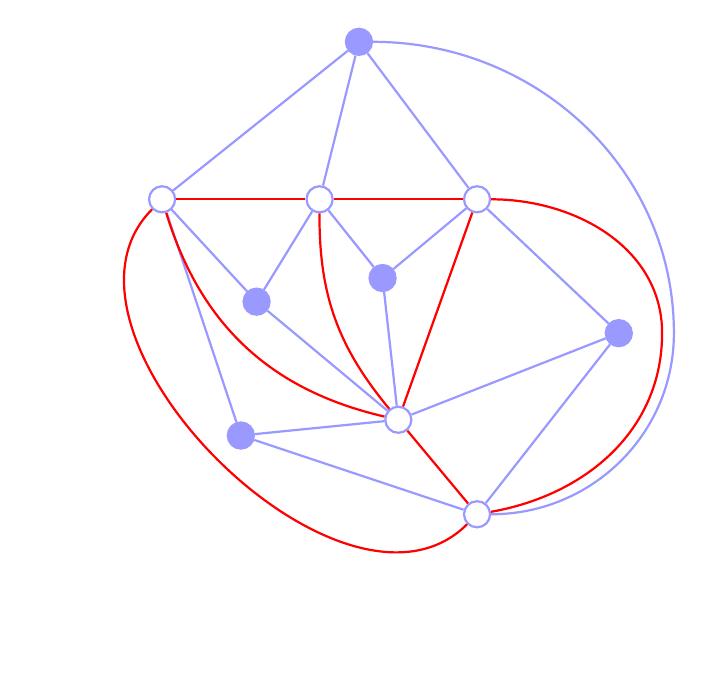
\begin{tikzpicture}[main/.style = {draw, circle, thick, Blue!40},
			edge/.style = {thick, Blue!40},
			fil/.style = {thick, fill, draw, circle, Blue!40},
			red/.style = {thick, Red}]
			\node[main] (1) at (0,0) {};
			\node[fil] (2) at (1.8, 2.3) {};
			\node[fil] (3) at (-3, 1) {};
			\node[main] (4) at (-1, 1.2) {};
			\node[fil] (5) at (-1.2, 3) {};
			\node[fil] (6) at (-2.8, 2.7) {};
			\node[main] (7) at (-4, 4) {};
			\node[main] (8) at (-2, 4) {};
			\node[main] (9) at (0, 4) {};
			\node[fil] (10) at (-1.5, 6) {};
			\draw[edge] (1) -- (2);
			\draw[edge] (1) -- (3);
			\draw[edge] (3) -- (4);
			\draw[edge] (2) -- (4);
			\draw[edge] (4) -- (5);
			\draw[edge] (4) -- (6);
			\draw[edge] (2) -- (9);
			\draw[edge] (9) -- (10);
			\draw[edge] (8) -- (10);
			\draw[edge] (7) -- (10);
			\draw[edge] (3) -- (7);
			\draw[edge] (6) -- (7);
			\draw[edge] (5) -- (8);
			\draw[edge] (6) -- (8);
			\draw[edge] (5) -- (9);
			\draw[edge] (1) to[out=0, in=270] (2.5, 2.3) to[out=90, in=0] (10);
			\draw[red] (1) edge (4);
			\draw[red, bend right = 30] (7) edge (4);
			\draw[red, bend left = 90] (1) edge (7);
			\draw[red, bend right = 20] (8) edge (4);
			\draw[red] (4) edge (9);
			\draw[red] (8) edge (9);
			\draw[red] (1) to[out=10, in=270] (2.35, 2.3) to[out=90, in=0] (9);
			\draw[red] (7) edge (8);
		\end{tikzpicture}
		\caption{The graph $G$.}
	\end{subfigure}
	\caption{An illustration to the proof of Theorem \ref{thm-3}.}
\end{figure}